\chapter{مبانی نظری}\label{chap3}
\setlength{\parindent}{2em}
\minitoc

در این فصل مبانی نظری‌ای که پایه‌ها و ستون‌های راهکار پیشنهادی ارائه شده هستند، بیان و تشریح می‌شوند. در اولین بخش از این فصل معماری ترنسفورمر ارائه خواهد شد. در بخش دوم، شبکه‌های از پیش آموزش داده شده ترنسفورمری نظیر برت و بارت ارائه خواهند شد. آخرین بخش نیز به بررسی بعضی معیارهای سنجش تولید متن پرداخته شده است.

\section{ترنسفورمرها}

تا قبل از پیدایش معماری ترنسفورمر غالب مدل‌های پردازش دنباله بر پایه‌ ساختار‌های پیچیده شبکه‌های بازگشتی و یا شبکه‌های 
\trans{پیچشی}{Convolutional}
بنا شده بودند و البته معمولا بهترین عملکرد این شبکه‌ها نیز در حالتی بود که شبکه‌های رمزگذار و رمزگشای خود را با مکانیزم توجه نیز به یکدیگر اتصال می‌دادند. 
مکانیزم توجه در واقع به قسمت رمزگشا این اجازه را می‌دهد تا در هنگام تولید هر کلمه در رشته خروجی بتواند راحت‌تر وابستگی متناظر با آن کلمه را در رشته ورودی کشف و استفاده کند. در حالتی که مکانیزم توجه وجود نداشته باشد به علت رمزشدن بازنمایی رشته ورودی در یک بردار با طول ثابت معمولا اطلاعات به سختی از قسمت رمزگذار به رمزگشا منتقل می‌شوند، حال آن که مکانیزم توجه با ایجاد اتصالات متعدد از رمزگذار به رمزگشا انتقال جریان اطلاعات از رمزگذار به رمزگشا و جریان مشتق از رمزگشا به رمزگذار را تسهیل کرده است.

ترنسفورمر
از نظر کارکردی در واقع یک مدل دنباله به دنباله رمزگذار-رمزگشا است که بدون استفاده از مکانیزم‌های بازگشتی صرفا بر مکانیزم توجه تکیه دارد
\cite{transformer}
. مدل‌های مبتنی بر ترنسفورمر اکنون پرچمدار
\trans{مرز دانش}{State of the Art}
بسیاری از زیرمسائل موجود در وظایف از جنس دنباله‌ای نظیر مدل‌زبانی
،
ترجمه ماشینی
، تشخیص موجودیت‌های اسمی، تحلیل احساسات
و بسیاری از زیرمسائل دیگر هستند.

ترنسفورمر به لحاظ ساختاری از دو زیرشبکه رمزگذار و رمزگشا تشکیل شده است.   
زیر شبکه رمزگذار آن جمله مبدا را در ورودی گرفته و یک بازنمایی از آن را تولید میکند. زیر شبکه رمزگشا نیز بازنمایی حاصل از زیر شبکه رمزگذار و همچنین کلمات تولید شود تا حال حاضر از جمله مقصد را گرفته و سعی در تخمین توزیع احتمال کلمه بعد دارد. در شکل 
\ref{fig:chap3:transfoermer_overview}
نمایی کلی از معماری ترنسفورمر آورده شده است. در ادامه اجزای مختلف ترنسفورمر تشریح شده‌اند.


\begin{figure}[h]
	\centering
	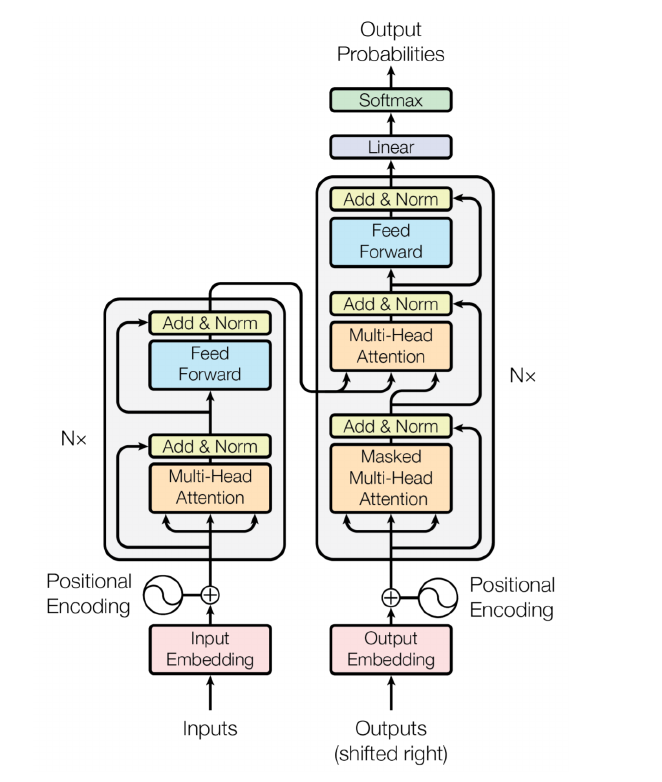
\includegraphics[width=0.85\textwidth]{images/chap3/transformer_arch.png}
	\caption{
		نمایی کلی از معماری ترنسفورمر
		\cite{transformer}
	}
	\label{fig:chap3:transfoermer_overview}
\end{figure}

\subsection{رمزگذار و رمزگشا}
قسمت رمزگذار ترنسفورمر از یک 
\trans{پشته}{Stack}
از چندین لایه یکسان تشکیل شده است که هر لایه خروجی خود را به عنوان ورودی به لایه بعدی تحویل می‌دهد. هر لایه پشته کدگذار دو بلوک وجود دارد. بلوک اول یک مکانیزم 
\trans{خودتوجه چندسر}{Multi-Head Self-Attention}
است و بلوک دوم نیز یک شبکه عصبی 
\trans{پیشرو}{Feed-Forward}
\trans{تمام متصل}{Fully connected}
است که مستقل از مکان عمل می‌کند. در ضمن در هر بلوک نیز از 
\trans{اتصالات باقی‌مانده}{Residual Connection}
و 
\trans{نرمال کننده لایه}{Layer Normalization}
استفاده می‌شود.

زیر شبکه رمزگشای ترنسفورمر نیز مانند رمزگذار دارای چندین لایه است با این تفاوت که هر لایه دارای سه بلوک است. بلوک اول و بلوک سوم رمزگشا دقیقا مانند بلوک های اول و دوم رمزگذار هستند. بلوک میانی اما در واقع نقش اتصال رمزگذار و رمزگشا را دارد و به وسیله یک توجه چند سر، مکانیزم توجه را روی خروجی آخرین لایه رمزگذار انجام می‌دهد. در ضمن یک تفاوتی که در بلوک اول رمزگذار با رمزگشا وجود دارد است که عمل توجه به خود در رمزگشا صرفا بر روی ورودی‌های قبل از توکنی که قصد توجه دارد انجام می‌شود.


\subsection{مکانیزم توجه در ترنسفورمر}

\subsubsection{تعمیم مکانیزم توجه}
در این پژوهش مکانیزم توجه به شکل تعمیم یافته‌ای ارائه شده است. در واقع در مکانیزم توجه تعمیم یافته سه جز اساسی بردار 
\trans{پرس و جو}{Query}
و یک جفت بردار‌های کلید-مقدار برای هر توکن در نظر گرفته می‌شوند. بردار خروجی مکانیزم توجه، حاصل جمع‌ وزن‌دار بردارهای مقدار  توکن‌های مورد توجه می‌باشد که این وزن‌ها خود تابعی از بردار 
پرس و جوی توکن در حال توجه و بردارهای کلید توکن‌های مورد توجه می‌باشند.

در روند پیاده‌سازی مکانیزم توجه در مدل ترنسفورمر از تابع ضرب داخلی به عنوان تابع محاسبه‌گر امتیاز مشابهت بردار‌های پرس و جو و کلید استفاده شده است.
سپس با اعمال تابع Softmax روی تمامی امتیاز‌های مشابهت متعلق به توجه یک بردار پرس و جو بر روی مجموعه ای بردارهای کلید، وزن مربوطه ترکیب خطی مکانیزم توجه محاسبه می‌گردد. در نهایت از آن‌جایی که به ازای مقادیر بزرگ 
$d_k$
که اندازه بردار کلید است، حاصل ضرب داخلی بسیار بزرگ می‌شود و خروجی تابع 
\lr{Softmax}
به گونه‌ای می‌شود که مشتق بسیار ضعیفی به عقب باز‌ می‌گردد، جهت رفع این مشکل، امتیازات قبل از اعمال 
\lr{Softmax}
تقسیم بر 
$\sqrt{d_k}$
می‌شوند. جهت درک بهتر این عملیات شکل
\ref{fig:chap3:transformer_attention}
 آورده شده است.

\begin{figure}[h]
	\centering
	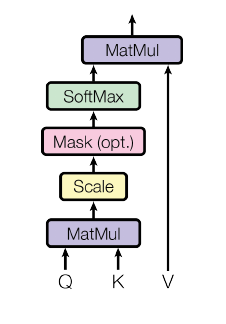
\includegraphics[width=0.3\textwidth]{images/chap3/transformer_attention.png}
	\caption{
		نمایی از مکانیزم توجه در مدل ترنسفورمر
		\cite{transformer}
	}
	\label{fig:chap3:transformer_attention}
\end{figure}

\subsubsection{مکانیزم توجه چندسر}

نکته جالب توجه دیگر در معماری ترنسفورمر مکانیزم توجه چندسر است. در مقاله این گونه بیان شده که به جای این که هر بار یک توجه با ابعاد بردار 
$d_{model}$
انجام بگیرد، می‌توان بردارهای پرس و جو، کلید و مقدار را با کمک شبکه‌های پیشرو قابل یادگیری به تعداد
$h$
فضای با ابعاد
$d_{model/h}$
تصویر کرد و سپس 
$h$
عمل توجه را روی این بردار‌های تصویر شده انجام داد و در نهایت حاصل این توجهات را با یکدیگر الحاق کرد. مکانیزم توجه چندسر به مدل اجازه می‌دهد تا همزمان بتواند به اطلاعاتی از فضاهای 
\trans{بازنمایی}{representation}
مختلفی توجه کند. به علاوه امکان موازی‌سازی بین این عملیات‌های توجه نیز فراهم است و از این حیث مدل دچار هزینه زمانی اضافی نمی‌شود. برای درک بهتر مکانیزم توجه چندسر شکل 
\ref{fig:chap3:transformer_multihead}
آورده شده است.
\begin{figure}[h]
	\centering
	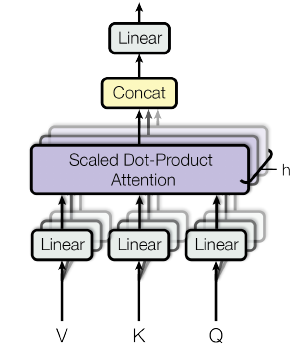
\includegraphics[width=0.4\textwidth]{images/chap3/transformer_multihead.png}
	\caption{
		نمایی از مکانیزم توجه در مدل ترنسفورمر
		\cite{transformer}
	}
	\label{fig:chap3:transformer_multihead}
\end{figure}


\subsubsection{موارد استفاده از توجه در ترنسفورمر}
مدل ترنسفورمر از مکانیزم توجه چندسر در سه موقعیت مختلف استفاده می‌کند:

\begin{itemize}
	\item 
	\textbf{توجه کدگشا به کدگذار}:
	در این بخش بردار‌های پرس و جو از لایه‌ی‌ قبلی کدگشا حاصل می‌شوند و بردارهای کلید و مقدار نیز از خروجی رمزگذار به دست می‌آیند.
	
	\item 
	\textbf{توجه به خود کدگذار}:
	در این بخش تمامی بردارهای پرس و جو و کلید و مقدار از خروجی لایه قبلی کدگذار حاصل می‌شوند. هر توکن در هر مکانی در کدگشا می‌تواند به تمامی توکن‌ها (چه قبل و چه بعد از خود) توجه کند.
	
	\item
	\textbf{توجه به خود کدگشا}:
	این مورد مانند توجه به خود کدگشا است، با این تفاوت که هر توکن در کدگشا تنها می‌تواند به بردارهای مقدار و کلید توکن‌های قبل از خود توجه کند.
	
	
\end{itemize}

\subsection{شبکه پیشرو تمام متصل مستقل از مکان}:
علاوه بر بلوک توجه، هر یک از لایه‌ها در کدگذار و کدگشا دارای یک بلوک شبکه عصبی تمام متصل پیشرو هستند. این شبکه به هر برداری در هر مکانی به صورت جدا و البته یکسان اعمال می‌شود (البته دقت شود که پارامتر‌های این شبکه‌های متصل لایه به لایه فرق می‌کنند). این شبکه یک شبکه با یک لایه مخفی است، اندازه بردارهای ورودی و خروجی آن ۵۱۲ می‌باشد و اندازه بردار حالت نهان آن هم ۲۰۴۸ است. کاربرد و فلسفه وجودی این شبکه در استخراج ویژگی از بردارهای حاصل از مکانیزم توجه است.


\subsection{
مکانیزم
\trans{تعبیه}{Embedding}
مکانی
}
از آنجایی که ساختار شبکه ترنسفورمر بازگشتی نمی‌باشد، بنابراین لازم است تا مکانیزمی جهت تزریق اطلاعات موقعیت مکانی کلمات دنباله نسبت به یکدیگر به مدل طراحی شود. به منظور حل این چالش در مدل ترنسفورمر برداری به نام بردار تعبیه مکانی در نظر گرفته شده است که بنابر رابطه
\ref{eq:positional_embedding}
به دست می‌آید.

\begin{align} \label{eq:positional_embedding}
PE_{(pos, 2i)} = sin(pos/10000^{2i/d_{model}}) \\  \nonumber
PE_{(pos, 2i+1)} = cos(pos/10000^{2i/d_{model}}) 
\end{align}

این بردار تعبیه مکانی با اندازه 
\lr{$d_{model}$}
 به ازای هر توکن با مکان مختلف که متغیر
\lr{pos}
می‌باشد تعریف می‌شود. در نهایت بردار تعبیه مکانی با بردار تعبیه کلمه جمع خواهد شد.

\subsection{علت اهمیت به معماری ترنسفورمری}
ترنسفورمر‌ها به علت توانایی موازی‌سازی عملیات‌های خود در هنگام آموزش نسبت به شبکه‌های بازگشتی، سریعتر آموزش می‌بینند. از طرفی وجود عملیات توجه به خود چه در رمزگذار و چه در رمزگشا نیز خود عاملی برای تقویت این مدل نسبت به مدل‌های بازگشتی استفاده کننده از توجه شده است و به صورت خاص به نظر می‌رسد که وجود این توجه به خود برای مساله گفتگو بسیار موثرتر از وجود مکانیزم توجه بدون توجه به خود است.

\section{نهضت انتقال یادگیری در پردازش زبان}
تولد پارادایم انتقال یادگیری را می‌توان مترادف با به وجود آمدن شبکه‌های غول آسایی نظیر
\LR{AlexNet}
و
\LR{VGG}
که بر روی دادگان عظیم تصویری آموزش یافته‌اند در نظر گرفت. محققان حوزه یادگیری عمیق و بینایی ماشین، با آموزش این مدل‌ها روی دادگان عظیم در پی این بودند که بتوانند بازنمایی‌های مناسبی از تصاویر به دست آورند؛ به نحوی که در روند حل مسائل دیگر بتوانند از آن‌ها به عنوان ویژگی‌ استفاده کنند. 

در حوزه متن اما اولین نمونه از انتقال یادگیری را می‌توان مدل معروف 
\lr{word2vec}
 ارائه شده توسط میکولوف در سال ۲۰۱۳ دانست
\cite{word2vec_paper}.
به این صورت که وظیفه حدس زدن کلمات اطراف یک کلمه توسط یک شبکه با یک لایه مخفی بر روی دادگان بسیار آموزش دیده شده و بازنمایی حاصل از آن شبکه به عنوان بازنمایی هر کلمه مدنظر قرار گرفت. پس از عرضه مدل 
\lr{word2vec}
مرز‌های دانش در بسیاری از مسائل پردازش زبان، بسیار فراتر از حد فعلی خود رفتند و این مدل کارایی خود را به نمایش گذاشت. اما از آن‌جایی که نقطه قوت این مدل از منظر انتقال یادگیری مورد توجه واقع نشد،‌ مسئله انتقال یادگیری نیز در حوزه پردازش زبان چند سال به خواب عمیقی فرو رفت تا آن که در سال ۲۰۱۸ مدل 
\lr{ELMO}
انتشار یافت. 

توضیح آن‌که با وجود این که شبکه‌هایی نظیر 
\lr{word2vec}
برای هر کلمه یک بردار بازنمایی مناسب تولید می‌کردند اما وجود کلمات چند معنایی مانند "شیر" و یا "بستر" (که می‌تواند به معنای بستر خواب یا بستر رودخانه باشد) محققین را به این فکر انداخت که بازنمایی یک کلمه بایستی تابعی از محتوایی که آن کلمه در آن قرار گرفته نیز باشد.  به فرض مثال بازنمایی کلمه "شیر" در دو عبارت "من شیر را خوردم" و یا "شیر سلطان جنگل است" بایستی متفاوت بوده و تابعی از جمله باشد. 

به طور اجمالی مدل 
\lr{ELMO}
از دو شبکه 
\lr{LSTM}
چند لایه تشکیل شده است که یکی از آن‌ها وظیفه 
\trans{مدل زبانی}{Language Model}
را از سمت چپ و دیگری نیز وظیفه 
مدل زبانی
را از سمت راست روی دادگان متنی آموزش می‌بینند. 
\footnote{
توضیح آن که یادگیری وظیفه مدل زبانی از دو سمت باعث می‌شود تا بازنمایی بهتری برای کلمات به وجود بیاید. برای مثال دو عبارت "من شیر جنگل را دیدم" را با "من شیر را همراه با کیک میخورم" مقایسه کنید. در صورتی که تنها از یک شبکه بازگشتی استفاده کنیم و جمله را از راست به چپ به شبکه بازگشتی ورودی بدهیم بازنمایی کلمه شیر در هر دو عبارت یکی خواهد بود.
}
در مرحله بعد، در صورتی که بخواهند از این شبکه به عنوان نقطه شروع و یا شبکه استخراج ویژگی از کلمات برای یک وظیفه دیگر استفاده کنند، ترکیب خطی قابل یادگیری از بازنمایی کلمات در لایه‌های مختلف هر دو
\lr{LSTM}
را به عنوان بازنمایی آن کلمه در نظر می‌گیرند. برای درک بهتر معماری ELMO در شکل 
\ref{fig:chap3:elmo_arch}
به نمایش درآمده است.

\begin{figure}[h]
	\centering
	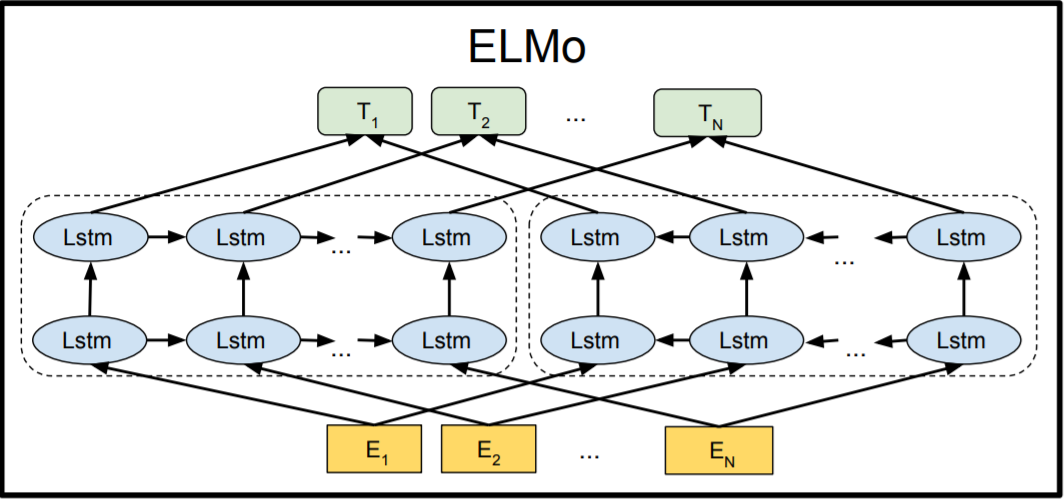
\includegraphics[width=0.8\textwidth]{images/chap3/elmo_arch.png}
	\caption{
		نمایی از معماری مدل المو
	}
	\label{fig:chap3:elmo_arch}
\end{figure}

 با ظهور مدل المو مرز‌های دانش در مسائل پردازش زبان گسترش پیدا کردند و امتیاز بهترین مدل‌ها در مسائل گوناگون پردازش زبان بهبود یافت. با این وجود به دلیل این که المو یک شبکه بازگشتی محسوب می‌شد، مشکلات شبکه‌های بازگشتی از قبیل توانایی کمتر در موازی‌سازی و همچنین انفجار یا ناپدید شدن گرادیان، در المو نیز وجود داشت.  

\subsection{مدل برت}
پس از ارائه معماری ترنسفورمر، توجهات در حوزه پردازش زبان از معماری‌های بازگشتی به معماری‌های ترنسفورمری معطوف گشت و در اغلب مسائل مهاجرت از معماری های بازگشتی به معماری‌‌ها نو شکل گرفت. 
طبعا این مهاجرت محققان این حوزه را نیز به این فکر انداخت تا مدلی با معماری ترنسفورمری و با کارکرد مشابه با المو ارائه دهند. سرانجام این ایده، منجر به انتشار مدل برت در سال ۲۰۱۹ گردید
\cite{bert}
.

مدل برت از لحاظ ساختاری، یک پشته رمزگذار ترنسفورمری محسوب می‌شود. 
\footnote{در واقع ترنسفورمری است که تنها قسمت رمزگذار را داراست و فاقد قسمت رمزگشا است.}
هدف مدل برت مشابه المو به دست آوردن یک بازنمایی از طریق آموزش روی دادگان فراوان متنی بدون برچسب است. مزیت ساختاری برت بر المو را نیز می‌توان اولا در سرعت بالاتر و آموزش راحت شبکه‌ ترنسفورمری نسبت به شبکه بازگشتی دانست و از آن مهم‌تر امکان توجه توامان
\trans{دوطرفه}{Bidirectional}
 در هر کلمه نسبت به محتوای سمت چپ و راست آن دانست. در واقع در مدل برت بردار بازنمایی یک کلمه می‌تواند به کلمات سمت راست و چپ خود همزمان توجه کند در حالی که در مدل المو ما با دو شبکه بازگشتی مواجه هستیم که هر یک سعی دارند به طور غیرتوام توجه بردار بازنمایی کلمه را به سمت چپ و راست معطوف کنند. 
 
 در مقاله برت دو طرح اساسی مطرح شده است. طرح اول، چگونگی پیش آموزش شبکه برت و طرح دوم نیز چگونگی تنظیم آن روی وظایف مختلف پردازش زبان است.
 
 \subsubsection{چگونگی پیش‌آموزش برت}
 به منظور پیش آموزش شبکه برت، دو وظیفه 
 \trans{مدل زبانی پوشیده}{Masked-Language-Model}
 و 
 \trans{تشخیص جمله بعدی}{Next Sentence Prediction}
 انتخاب شده اند.
در مسئله مدل زبانی پوشیده، بر خلاف مسئله مدل زبانی عادی که در آن هدف یادگیری
\trans{توزیع احتمال}{Probability Distribution}
کلمه از روی کلمات قبلی اش است، هدف یادگیری توزیع اجتمال یک کلمه از روی کلمات قبل و بعد از خودش است. طبیعی است که با توجه به اهتمام برت بر به دست آوردن یک بازنمایی دوطرفه توامان وظیفه مدل زبانی پوشیده جهت نیل به این هدف بسیار موثر تر از وظیفه مدل زبانی عادی است. در هنگام پیش آموزش برت با وظیفه مدل زبانی پوشیده، به تصادف ۱۵ درصد از کلمات دنباله با توکن 
\lr{MASK}
تعویض می‌شوند و مدل بایستی بتواند که کلمه اول توکن‌های پوشیده شده را تشخیص دهد. 

با این که آموزش روی وظیفه مدل زبانی پوشیده به برت کمک می‌کند برای هر کلمه بازنمایی موثری بیابد اما برت برای انجام برخی تسک‌های پردازش زبان نیاز به ارائه بازنمایی مناسبی از جملات
و همچنین شف رابطه بین جملات مختلف،
 نیز دارد. به این منظور، برت پس از پیش آموزش مدل زبانی پوشیده، روی وظیفه جدس جمله بعدی نیز آموزش می‌بیند. صورت این مساله این شکلی است که جمله A از دادگان آموزشی انتخاب می‌شود. سپس به احتمال پنجاه درصد جمله پس از A به عنوان جمله B انتخاب می‌شود و یا به احتمال باقی مانده پنجاه درصد یک جمله تصادفی به عنوان جمله B انتخاب می‌شود. سپس مدل بایستی این که آیا جمله B جمله بعدی جمله A است یا خیر را حدس بزند. 

 در پیاده‌سازی برت، هنگام ورود یک رشته در ابتدای آن یک توکن
\lr{[CLS]}
اضافه می‌شود که بردار بازنمایی حاصل آن از شبکه برت، بردار بازنمایی جمله را ارائه می‌دهد و در وظیفه تشخیص جمله بعدی، یک لایه
\lr{Softmax}
روی بردار بازنمایی
\lr{[CLS]}
اضافه گشته و احتمال خواسته شده را به دست می‌آورد. همچنین در پایان هر جمله نیز توکن
\lr{[SEP]}
اضافه می‌شود که جهت نشان دادن اتمام جمله ها به مدل به کار می‌رود. علاوه بر این، بردار
\trans{تعبیه قطعه‌ای}{Segment Embedding}
قابل یادگیری نیز با دو مقدار مختلف به دو جمله اول و دوم اعمال می‌شود. در واقع برت دارای سه مکانیزم تعبیه مکانی، قطعه‌ای و کلمه‌ای است که به ترتیب بر رشته ورودی اعمال می‌شود. جهت درک بهتر این تعبیه‌سازی‌ها، شکل
\ref{fig:chap3:bert_embeddings}
 آورده شده است.

 \begin{figure}[h]
 	\centering
 	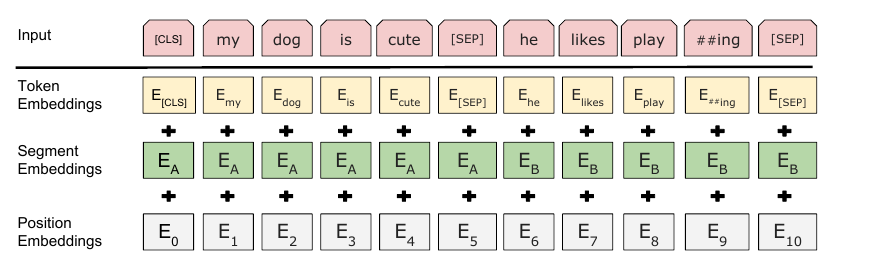
\includegraphics[width=1\textwidth]{images/chap3/bert_embeddings.png}
 	\caption{
 		نمایی از انواع تعبیه در مدل برت
 	}
 	\label{fig:chap3:bert_embeddings}
 \end{figure}

حسن و مزیت مسائل پیش آموزش برت در این است که دادگان بی برچسب موردنیاز آن‌ها به آسانی قابل جمع آوری است و همین باعث شده است که در طی دوره کوتاهی مدل برت 
توسط افراد مختلف
برای زبان‌های دیگر (از جمله فارسی) نیز آموزش یافته و در اختیار عموم قرار گیرد. 

\subsubsection{نحوه تنظیم برت برای وظایف مختلف}
در مقاله برت،‌ پس از مشخص‌شدن نحوه پیش آموزش این شبکه، معماری‌های پیشنهادی مبتنی بر برت برای حل بعضی از مسائل پردازش زبان نظیر تحلیل احساسات، تشخیص موجودیت‌های اسمی و پرسش و پاسخ ارائه شده است. رویکرد حل این مسائل با برت به این نحو است که معمولا لایه‌هایی جهت حل مساله مورد نظر به برت پیش آموزش یافته اضافه می‌شوند و معماری جدید (که برت پیش‌آموزش یافته حالا جزیی از آن است) روی مساله مورد نظر و دادگان برچسب‌دار آن تنظیم می‌شود. 

\subsection{مدل‌های پس از برت}
با این که با عرضه برت، یک انقلاب در حوزه پردازش زبان و مسائلش رخ داد و مرز‌های دانش بسیاری از مسائل با استفاده از معماری‌های مبتنی بر برت پیشرفت قابل توجهی را تجربه کردند؛ اما برت بی عیب و نقص نیست و راه‌حل تمامی مسائل پردازش زبان نیست محسوب نمی‌شود. به دلیل ضعف‌های نسبی برت و همچنین موفقیت چشم‌گیر آن بسیاری از پژوهشگران نیز در ادامه کوشیدند تا شبکه‌های از پیش آموزش یافته دیگری که بر پایه معماری ترنسفورمر باشند، را پیش آموزش داده و عرضه کنند.
از مهم‌ترین این شبکه‌ها بایستی به سری شبکه‌های 
\lr{GPT}
اشاره کرد که با انتشار خود، باعث پیشروی مرز‌های دانش در حوزه مسائل تولید زبانی شدند و حتی با خروجی‌های شگفت انگیز خود همگان را حیرت زده کردند.
و یا می‌توان به شبکه
\lr{Transformer-XL}
اشاره کرد که سعی دارد با اندکی تغییر در ساختار ترنسفومر، مشکل محدودیت برت 
(برت تنها می‌تواند متونی با حداکثر طول ۵۱۲ توکن را رمزکند)
در طول متون ورودی را حل کند. 

با وجود همه این پیشرفت‌ها و حتی به راه افتادن رقابت بین شرکت‌های بزرگ دنیا بر سر آموزش دادن یک مدل بزرگتر و با تعداد پارامتر بیشتر، اما به نظر می‌رسد در طول این رشد و رقابت روزافزون بین مدل‌های از پیش آموزش یافته، غفلتی نسبت به بخشی از ایده اصلی ترنسفورمر‌ها صورت گرفته است. تمامی شبکه‌های از پیش آموز‌ش‌یافته ارائه شده تا قبل از مدل برت، را می‌توان تنها متشکل از یک پشته رمزگذار معماری ترنسفورمر دانست. حتی تحت تاثیر این اتفاق، معماری‌های ارائه شده مبتنی بر این شبکه‌های از پیش آموزش یافته برای مسائل با ذات دنباله به دنباله نظیر مکالمه نیز، حالت دنباله به دنباله خود را از دست دادند و به صورت مدل زبانی مدل شدند
\cite{zhang2019dialogpt}.


\subsection{مدل بارت}
در حالی که بسیاری از محققین در حال صرف هزینه و تمرکز بر روی ایجاد مدل‌های تک پشته‌ای بودند، معماری دنباله به دنباله با عرضه مدل 
\lr{Bart}
دوباره مورد توجه واقع شد. 


\section{تکنیک عصاره‌گیری دانش}
